\setbeamercolor{background canvas}{bg=fitblue}
\begin{frame}
\frametitle{Color / Barva}
\begin{center}
\Huge {\color{white}Color / Barva}
\end{center}
\end{frame}
\setbeamercolor{background canvas}{bg=white}


\begin{frame}
    \frametitle{Color / Barva}
    \begin{columns}[c]
    \column{.5\textwidth}
        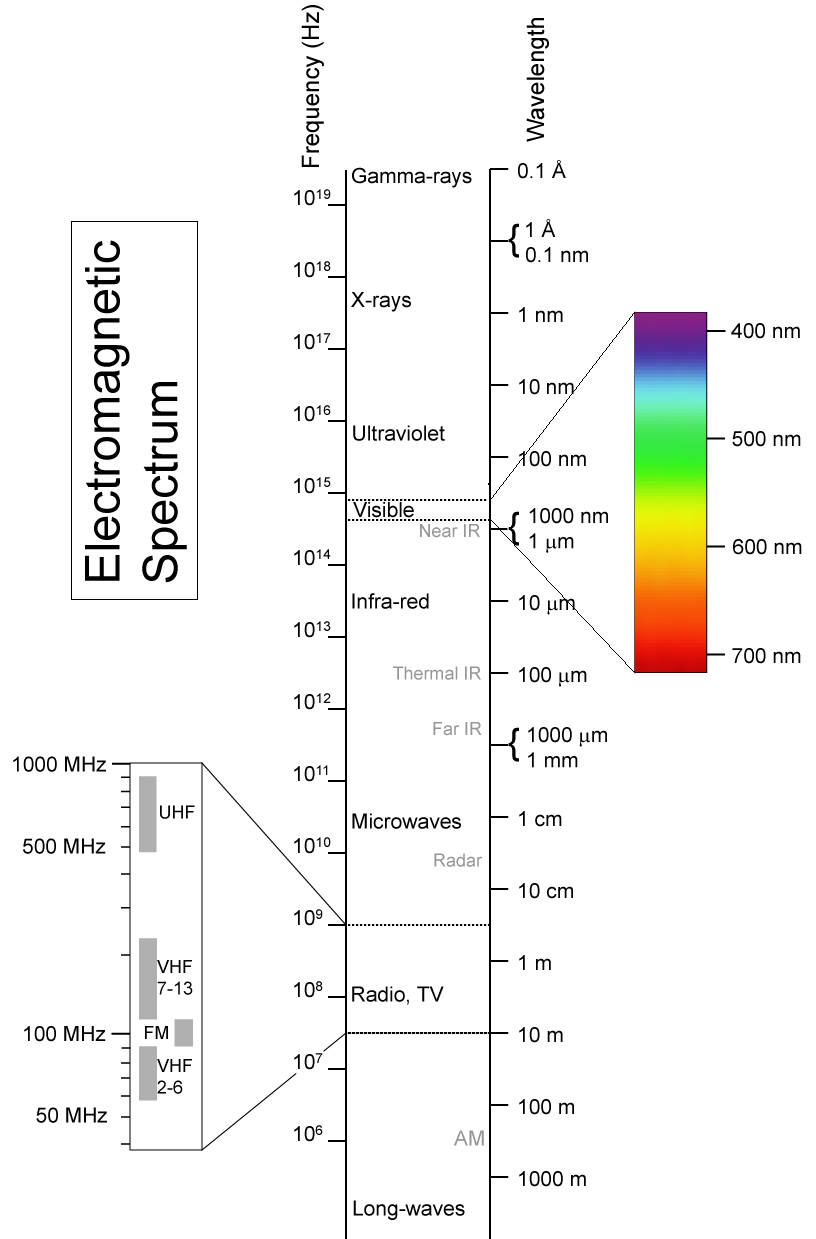
\includegraphics[height=\textheight]{pics/color/Electromagnetic-Spectrum}
    \column{.5\textwidth}
        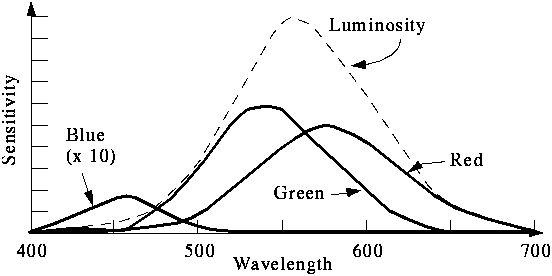
\includegraphics[width=\textwidth]{pics/color/citlivost-oka}

        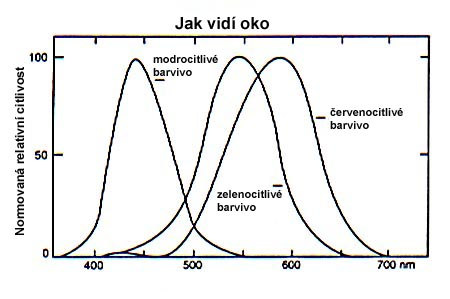
\includegraphics[width=\textwidth]{pics/color/citlivost-oka-normovana}
    \end{columns}
\end{frame}

\begin{frame}
    \frametitle{Gamut}
    \begin{columns}[c]
    \column{.5\textwidth}
        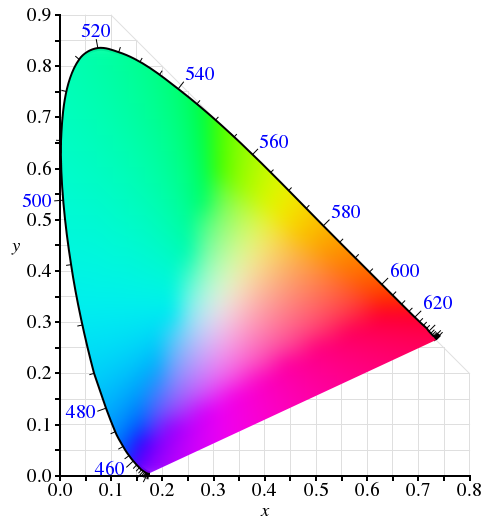
\includegraphics[width=\textwidth]{pics/color/gamut}
    \column{.5\textwidth}
        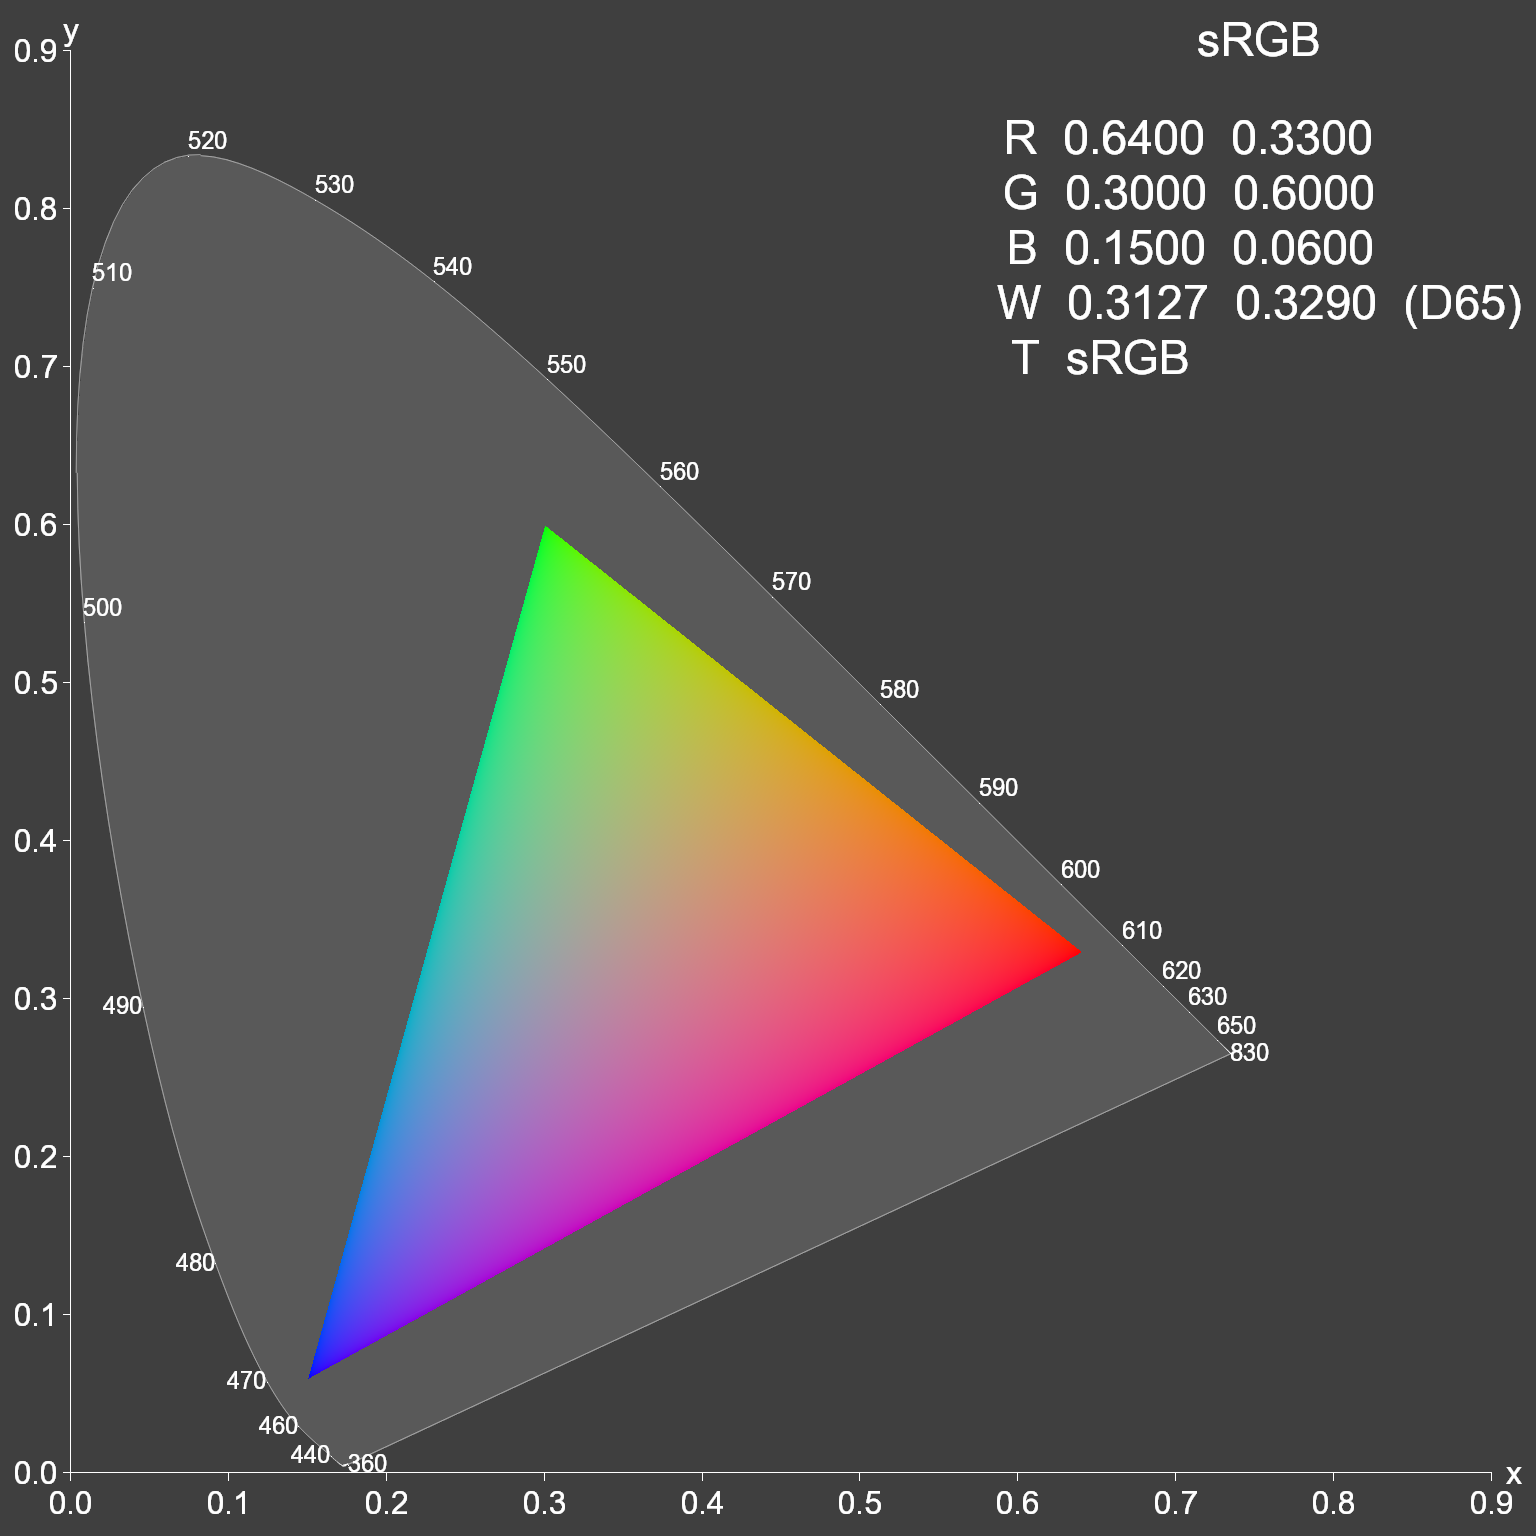
\includegraphics[width=\textwidth]{pics/color/Gamut-sRGB}
    \end{columns}
    \vfill
    \begin{itemize}
        \item CIE 1931
        \item XYZ vs RGB
    \end{itemize}
\end{frame}

\begin{frame}
    \frametitle{Gamma}

    \begin{columns}[c]
    \column{.5\textwidth}
        \scriptsize
        Logarithmic sensitivity of human eye\\
        Logaritmická citlivost oka

        \begin{eqnarray*}
        C_\mathrm{srgb}=\begin{cases}
        12.92C_\mathrm{l}, & C_\mathrm{l} \le t\\
        (1+a)C_\mathrm{l}^{\frac{1}{2.4}}-a, & C_\mathrm{l} > t
        \end{cases} \\
        a = 0.055 \\
        t = 0.0031308
        \end{eqnarray*}
        
    \column{.5\textwidth}
        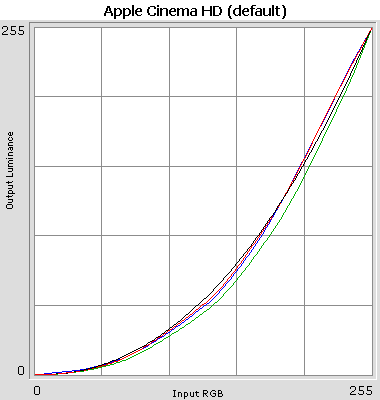
\includegraphics[width=\textwidth]{pics/color/monitor}
    \end{columns}
\end{frame}

\begin{frame}[fragile]
    \frametitle{Colors in OpenGL / Barva v OpenGL}

    Pipeline :
    \begin{itemize}
        \item float RGB(A) (vec3)
        \item {\color{black}$(0,0,0)$ \color{red}$(1,0,0)$ \color{green}$(0,1,0)$ \color{blue}$(0,0,1)$}
        \item[\color{red}!] Linear Color space, interpolation, blending.
    \end{itemize}
    \pause\vfill
    Vstupy a framebuffer :
    \begin{itemize}
        \item The most common RGB8
        \item Others : RGB16, RGB565, ...
        \item Linear or sRGB
        \item Conversion by hand?
    \end{itemize}
\begin{minted}[bgcolor=bg]{packages/c_cpp.py:CppLexer -x}
//default framebuffer
SDL_GL_SetAttribute(SDL_GL_FRAMEBUFFER_SRGB_CAPABLE,1);
...
//enabling SRGB in OpenGL
glEnable(GL_FRAMEBUFFER_SRGB);
\end{minted}
\end{frame}

\begin{frame}[fragile]
\frametitle{Gamma Correct}
  \scriptsize
	\begin{itemize}
  \item The light computation has to be done in linear space.
  \item After the computation is done, it has to be gamma corrected.
  \item Sharp transition from lit and shadowed parts.
	\end{itemize}
	\begin{itemize}
  \item Výpočet osvětlení musí být proveden v lineárním prostoru.
  \item Po výpočtu osvětlení je nutné obrázek upravit gamma korekcí.
  \item Ostrý přechod ze světla do stínu je správně.
	\end{itemize}
	\begin{figure}[h]
	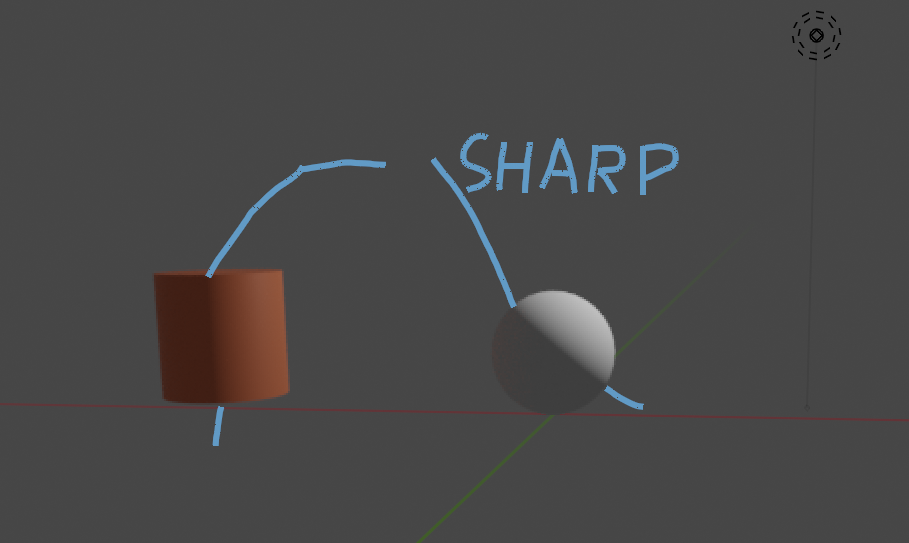
\includegraphics[width=8cm,keepaspectratio]{pics/color/gamma_correct}
	\end{figure}
\end{frame}

\begin{frame}[fragile]
\frametitle{Real Image}
	\begin{figure}[h]
	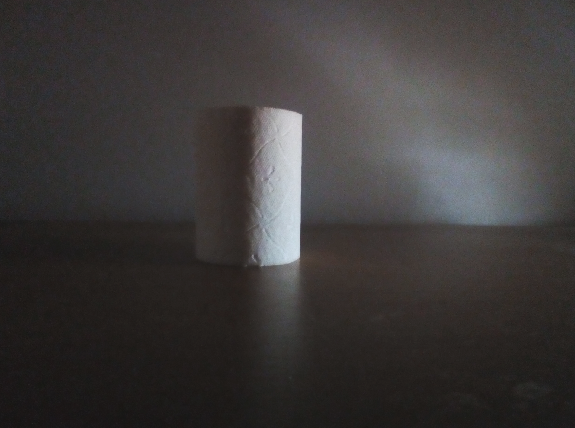
\includegraphics[width=8cm,keepaspectratio]{pics/color/gamma_real}
	\end{figure}
\end{frame}

\begin{frame}[fragile]
\frametitle{Gamma Correct}
	\begin{itemize}
  \item Left incorrect, right correct.
	\end{itemize}
	\begin{itemize}
  \item Vlevo bez korekce, vpravo s korekcí.
	\end{itemize}
	\begin{picture}(120,150)
		\put(0,0){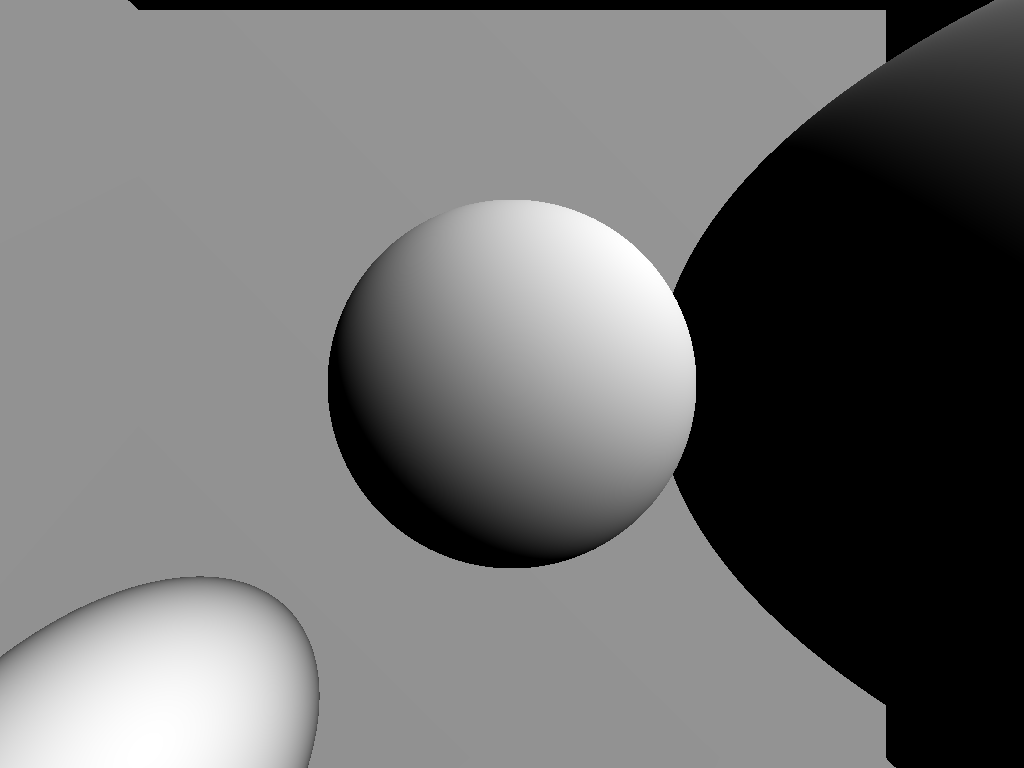
\includegraphics[width=6cm,keepaspectratio]{pics/color/no_correction}}
	\end{picture}
	\begin{picture}(60,40)
		\put(50,0){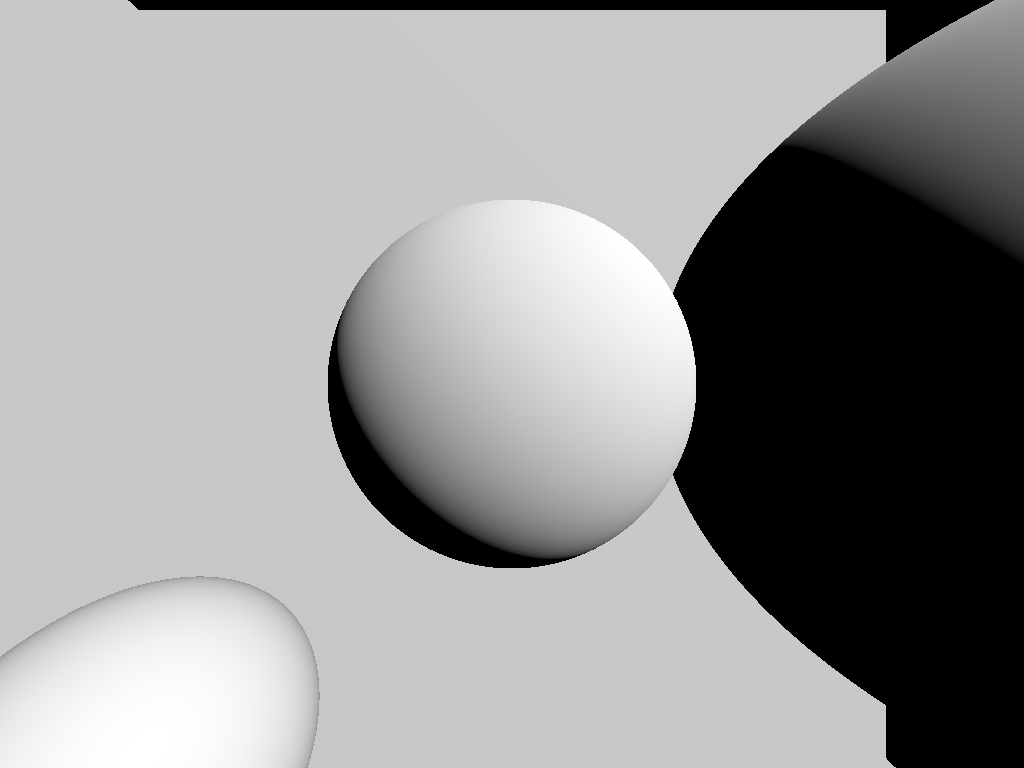
\includegraphics[width=6cm,keepaspectratio]{pics/color/correction}}
	\end{picture}
\end{frame}
